
\section{Intersections, intention and scenarios}
\label{sec:intro_intersections}
When it comes to the scenarios considered in this work. This section aims to clarify the use of the words' intersection, intention and scenario.
% When a pedestrian approach a crossing they have been taught at a young age to look at both sides of the road before crossing. The same apply for a human driver approaching an intersection. 
% When a human driver approach an intersection, it is natural to observe the environment to identify the traffic light, signs and other approaching vehicles. Then assess the situation, who has the right of way? 

% The intention of the other driver can be guided by the 
% Recently nontraditional intersections are also becoming increasingly popular. The goal of these designs is to reduce the number and/or severity of conflict points by altering the customary vehicular paths at the intersection. In light of the increased focus on and occurrence of these intersection types, it is expected that the application of nontraditional designs will continue to spread.

\begin{figure}[h]
	\centering
	\begin{subfigure}[t]{0.48\columnwidth}
		\centering
		\begin{tikzpicture}
			% Crossing
			\def\crossleftx{-2}
			\def\crossrightx{2}
			\def\crosstopy{2}
			\def\crossboty{-2}
			\def\roadwidth{0.5}

			\draw (0,0) circle (2pt);
			\node at (1.2, 0.2) {conflict point};
			\draw[thick] (\crossleftx, \roadwidth) -- (-\roadwidth, \roadwidth) -- (-\roadwidth, \crosstopy);
			\draw[thick] (\crossleftx, -\roadwidth) -- (-\roadwidth, -\roadwidth) -- (-\roadwidth-\roadwidth, \crossboty);
			\draw[thick] (\roadwidth, \crosstopy) -- (\roadwidth, \roadwidth) -- (\crossrightx, \roadwidth);
			\draw[thick] (\roadwidth-\roadwidth, \crossboty) -- (\roadwidth, -\roadwidth) -- (\crossrightx, -\roadwidth);

			% 	cars
			\node[inner sep=0pt] (ego_car) at (\crossleftx+0.5,0)
			{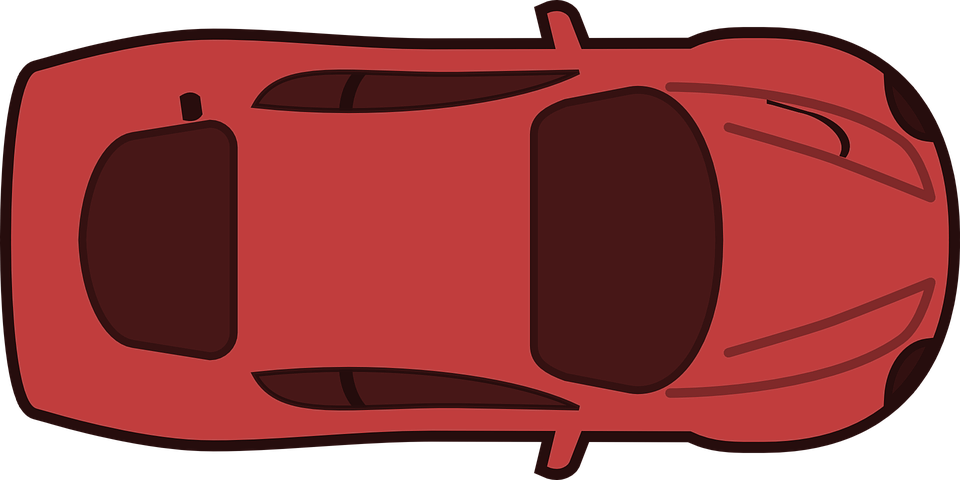
\includegraphics[width=.18\textwidth, angle=0]{figures/ego_car_top_down.png}};

			\node[inner sep=0pt] (target_car) at (0,\crosstopy-0.5)
			{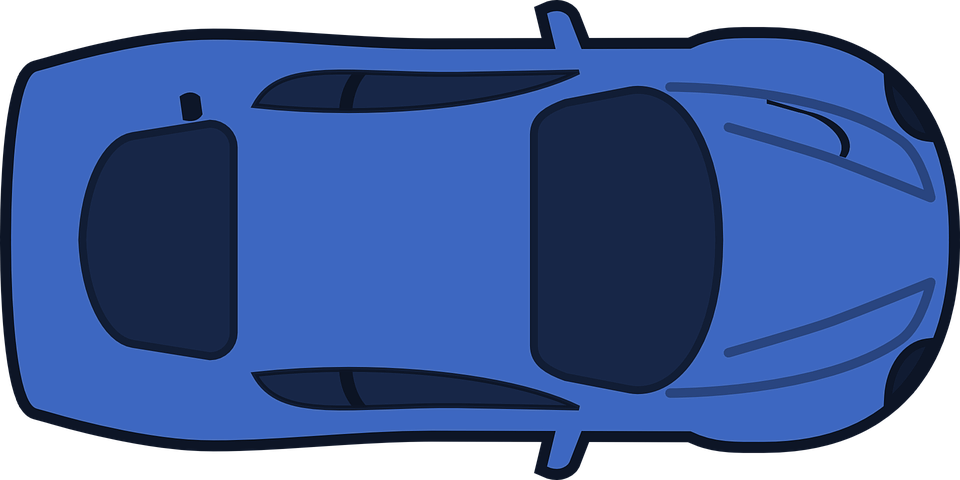
\includegraphics[width=.18\textwidth, angle=-90]{figures/target_car_top_down.png}};

			\node[inner sep=0pt] (target_car) at (-.1,-0.8)
			{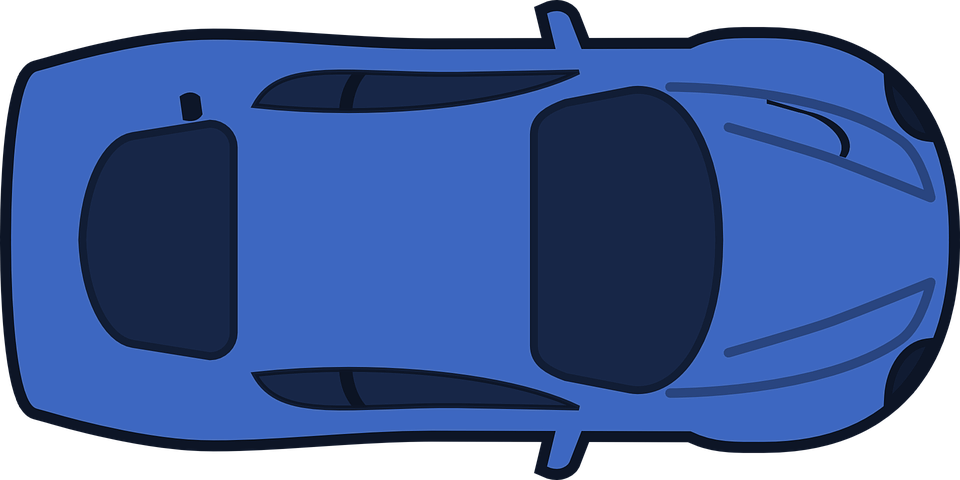
\includegraphics[width=.18\textwidth, angle=-110]{figures/target_car_top_down.png}};


		\end{tikzpicture}
		\label{fig:single_intersection}
		\caption{Single intersection}
\end{subfigure}%
	~ 
	\begin{subfigure}[t]{0.48\columnwidth}
		\centering
		\begin{tikzpicture}
			% Crossing
			\def\crossleftx{-2.5}
			\def\crossrightx{2.5}
			\def\crosstopy{2}
			\def\crossboty{-2}
			\def\roadwidth{0.5}

			\draw (-0.5,0) circle (2pt);
			\draw (0.5,0) circle (2pt);
			% \node at (0.7, 0.2) {crossing point$^1$};
			\draw[thick] (\crossleftx, \roadwidth) -- (-\roadwidth-0.5, \roadwidth) -- (-\roadwidth-0.5, \crosstopy);
			\draw[thick] (\crossleftx, -\roadwidth) -- (-\roadwidth-0.5, -\roadwidth) -- (-\roadwidth-0.5, \crossboty);
			\draw[thick] (0, \crosstopy) -- (0, \roadwidth);
			\draw[thick] (0, -\roadwidth) -- (0, \crossboty);
			\draw[thick] (\roadwidth+0.5, \crosstopy) -- (\roadwidth+0.5, \roadwidth) -- (\crossrightx, \roadwidth);
			\draw[thick] (\roadwidth+0.5, \crossboty) -- (\roadwidth+0.5, -\roadwidth) -- (\crossrightx, -\roadwidth);

			% 	cars
			\node[inner sep=0pt] (ego_car) at (\crossleftx+0.5,0)
			{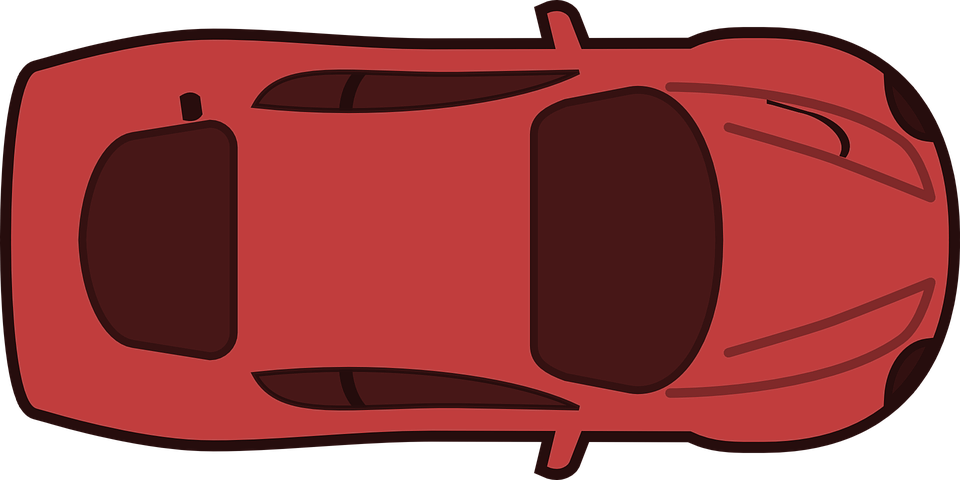
\includegraphics[width=.18\textwidth, angle=0]{figures/ego_car_top_down.png}};

			\node[inner sep=0pt] (target_car) at (-0.5,\crosstopy-0.5) {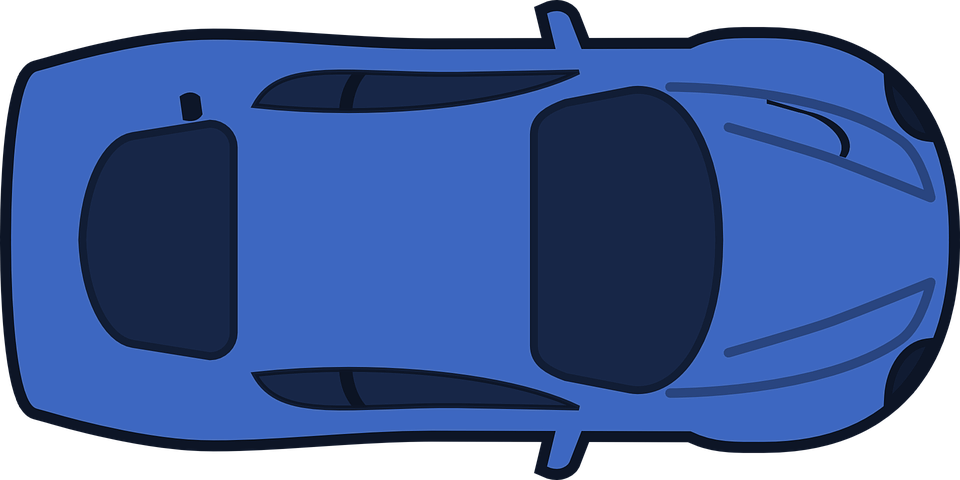
\includegraphics[width=.18\textwidth, angle=-90]{figures/target_car_top_down.png}};

			\node[inner sep=0pt] (target_car_2) at (0.5,\crossboty+0.5) {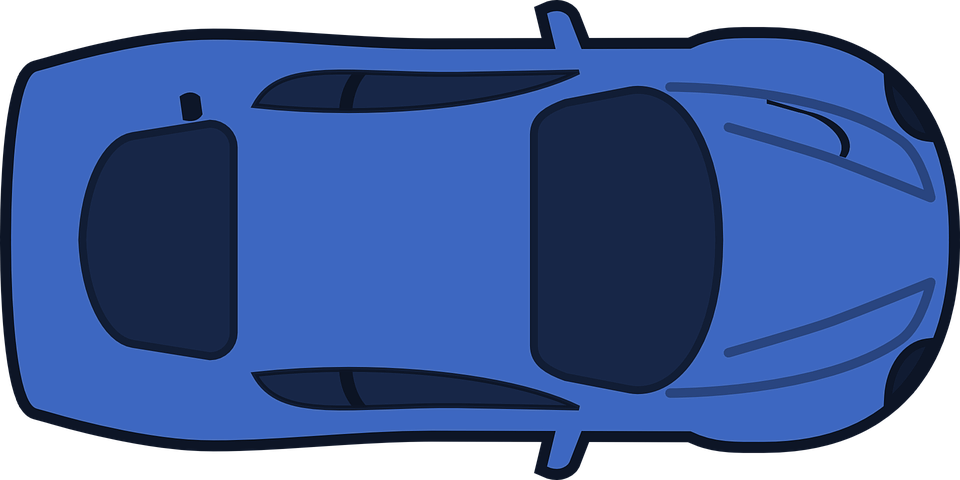
\includegraphics[width=.18\textwidth, angle=90]{figures/target_car_top_down.png}};

		\end{tikzpicture}
		\label{fig:double_intersection}

		\caption{Double intersection}
	\end{subfigure}

	\caption{Examples of different intersections}
	\label{fig:example_intersections}
\end{figure}
Let's begin by defining the terms \textit{intersection}, \textit{intention}, and \textit{scenario} within the context of this thesis.
An intersection refers to the geometric layout of roads intersecting each other, encompassing elements such as the number of junctions, conflict points, turns, and angles of incidence, as illustrated in Figure~\ref{fig:example_intersections}. 
Intersections can be categorized as signalized or unsignalized. A signalized intersection is equipped with infrastructure to designate the right-of-way, such as regulatory signs (e.g., STOP or YIELD) or traffic signals, while an unsignalized intersection lacks such features. However, as emphasized in the introduction, human drivers do not always follow these right-of-way rules, which can result in accidents. Therefore, this thesis defines intentions as the anticipated actions of other vehicles in the future, such as stopping or proceeding through the intersection.

\begin{figure}[h]
	% \mbox{\parbox{\textwidth}{
	% \centering
	% % \vspace{0.3cm}
	% 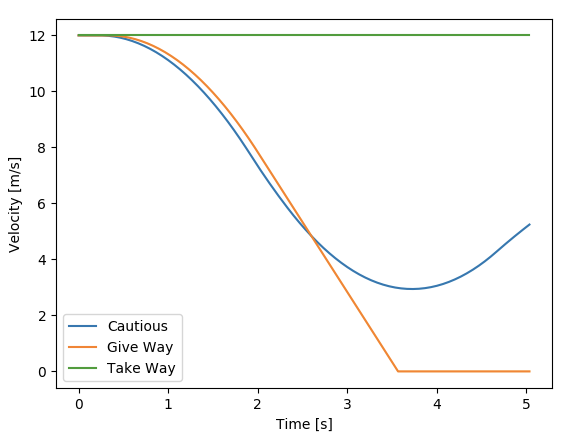
\includegraphics[width=0.6\columnwidth]{YourThesis/papers/mpc/figures/velocity_profiles_agents.png}
	% }}
	\centering
	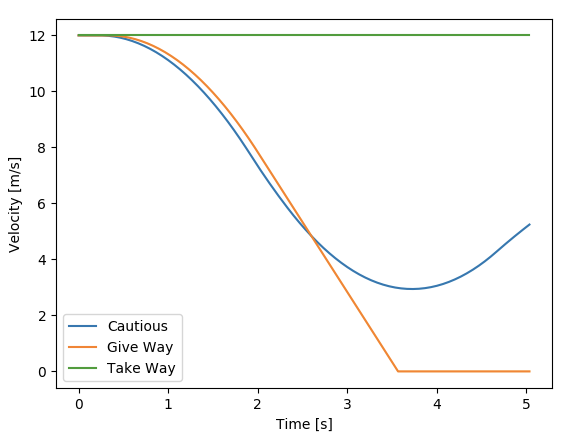
\includegraphics[width=0.6\columnwidth]{YourThesis/papers/mpc/figures/velocity_profiles_agents.png}

	\caption{An illustration showing velocity profiles for agents with three distinct intentions. Each agent shares the same initial position and velocity while approaching a common intersection.}
	\label{fig:intro_intention_profiles}
	% \vspace{-0.3cm}
\end{figure}

% Lets assume there are two main intentions, "take way" and "give way". However, it can be hard to distinguish between them, referring to Fig. 1..2.

Assume there are two main intentions: "take way" and "give way" (yield). In Figure \ref{fig:intro_intention_profiles}, three different agents with a starting velocity $12\mathrm{m/s}$ are approaching an intersection. At time $0$s, agents with a give way intention will start to brake. With these two main intentions, other intentions can be derived; for example, a cautious intention can be modeled as a give way agent that changes its intention to take way at 2 seconds. Distinguishing between the 'give way' and 'take way' intentions poses a challenge because even after the initial braking at 0 seconds, it is not certain that the agent will stop until 3 seconds after the initial braking. This uncertainty may be considered too conservative by the person riding the \gls{av}. 

% \tommy{A hypothesis is that the intention of a driver approaching an intersection can be derriverd by its way of driving towards the intersection.}
If intentions are known, intersections can be treated as unsignalized, as the right-of-way can be inferred from the intentions rather than relying solely on infrastructure. A \gls{rl} approach has the potential to improve driving in situations where it is beneficial to know the intention, such as when an intersection has both a stop sign and a traffic light or when another vehicle disregards traffic rules, like running a red light. By placing an \gls{rl} agent in a simulation environment with different driver intentions, it can infer the necessary information and take the best action based on trail and error. 
